\documentclass[a4paper,11pt]{report}
\usepackage[top=2cm,bottom=2cm,left=2cm,right=2cm]{geometry}
\usepackage[utf8]{inputenc}
\usepackage[frenchb]{babel}

\usepackage{multirow}
\usepackage{makecell}
\usepackage{fancyhdr}
\usepackage{caption}
\usepackage[final]{pdfpages}
\usepackage{tikz,pgfplots,pgf}
\usepackage{subcaption}
\usepackage{siunitx}
\usepackage[toc,page]{appendix}
\renewcommand{\appendixtocname}{Annexes}
\renewcommand{\appendixpagename}{Annexes}
\usepackage{tcolorbox, listings} 
\usepackage{sectsty}
\usepackage[french]{minitoc} 
\usepackage{hyperref}
\usepackage{titlesec}
\usepackage{colortbl}



\hypersetup{
	colorlinks=true, %colorise les liens
	breaklinks=true, %permet le retour à la ligne dans les liens trop longs
	urlcolor= blue,  %couleur des hyperliens
	linkcolor= black, %couleur des liens internes
	plainpages=false  %pour palier à "Bookmark problems can occur when you have duplicate page numbers, for example, if you have a page i and a page 1."
}


% Define a custom style
\lstdefinestyle{myC}{
    backgroundcolor=\color{backcolour},   
    commentstyle=\color{codegreen},
    otherkeywords={uint8_t, uint16_t, uint32_t, uint64_t, int8_t, int16_t, int32_t, int64_t, LiquidCrystal, BMP180, SHT21, DS1307, SI7034, WebUI, tm, MyTime, WiFi, Serial},
    keywordstyle=\color{codeblue},
    numberstyle=\tiny\color{codegray},
    stringstyle=\color{codeorange},
    basicstyle=\ttfamily\footnotesize,
    breakatwhitespace=false,         
    breaklines=true,                 
    keepspaces=true,                 
    numbers=left,       
    numbersep=5pt,                  
    showspaces=false,                
    showstringspaces=false,
    showtabs=false,                  
    tabsize=2,
}

\lstdefinestyle{myJava}{
    backgroundcolor=\color{backcolour},   
    commentstyle=\color{codegreen},
    otherkeywords={var, function, setInterval},
    keywordstyle=\color{codeblue},
    numberstyle=\tiny\color{codegray},
    stringstyle=\color{codeorange},
    basicstyle=\ttfamily\footnotesize,
    breakatwhitespace=false,         
    breaklines=true,                 
    keepspaces=true,                 
    numbers=left,       
    numbersep=5pt,                  
    showspaces=false,                
    showstringspaces=false,
    showtabs=false,                  
    tabsize=2,
}

\lstset{
  backgroundcolor=\color{backgroundColour},   
  commentstyle=\color{pGreen},
  keywordstyle=\color{pBlue},
  numberstyle=\tiny\color{pGray},
  stringstyle=\color{pOrange},
  basicstyle=\footnotesize,
  breakatwhitespace=false,         
  breaklines=true,                 
  captionpos=b,                    
  keepspaces=true,                 
  numbers=left,                    
  numbersep=5pt,                  
  showspaces=false,                
  showstringspaces=false,
  showtabs=false,                  
  tabsize=2,
  language=C,
  literate=
  {é}{{\'e}}1
  {è}{{\`{e}}}1
  {ê}{{\^{e}}}1
  {û}{{\^{u}}}1
  {ù}{{\`{u}}}1
  {â}{{\^{a}}}1
  {à}{{\`{a}}}1
  {ç}{{\c{c}}}1
  {Ç}{{\c{C}}}1
  {ô}{{\^{o}}}1
}


\chapterfont{\color{Pantone2377C}{}\fontfamily{pag}}
\sectionfont{\color{subtitlecolour}{}\fontfamily{pag}}
\subsectionfont{\color{subtitlecolour}{}\fontfamily{pag}}
\subsubsectionfont{\color{subtitlecolour}{}\fontfamily{pag}}

\definecolor{Pantone2377C}{HTML}{2C5574}
\definecolor{subtitlecolour}{HTML}{2C5574}
\definecolor{codegreen}{rgb}{0,0.6,0}
\definecolor{codegray}{rgb}{0.5,0.5,0.5}
\definecolor{codeblue}{HTML}{3E8BC0}
\definecolor{codeorange}{HTML}{ffa334}
\definecolor{codemauve}{HTML}{6A0888}
\definecolor{backcolour}{HTML}{efefef}





% Entête et pied de page
\pagestyle{fancy}
\rhead{
\includegraphics [scale=0.03, keepaspectratio=true]{img/ensta_logo_noir.png}}
\chead{}
\lhead{\leftmark }
\lfoot{Tanguy ROUDAUT - Tom ALLAIN}
\rfoot{FIPA SE 2024}
\cfoot{\thepage}
\renewcommand{\headrulewidth}{0.4pt}
\renewcommand{\footrulewidth}{0.4pt}




\titleformat{\chapter}[hang]{\bf\huge\color{Pantone2377C}}{Partie \thechapter}{2pc}{}
\begin{document}

% Page de couverture

\includepdf{pdf/page_de_garde.pdf}

% table des matieres
\tableofcontents

\clearpage
\chapter{Proteus}

    \section{Schéma}

        \begin{figure}[!h]
            \begin{center}
                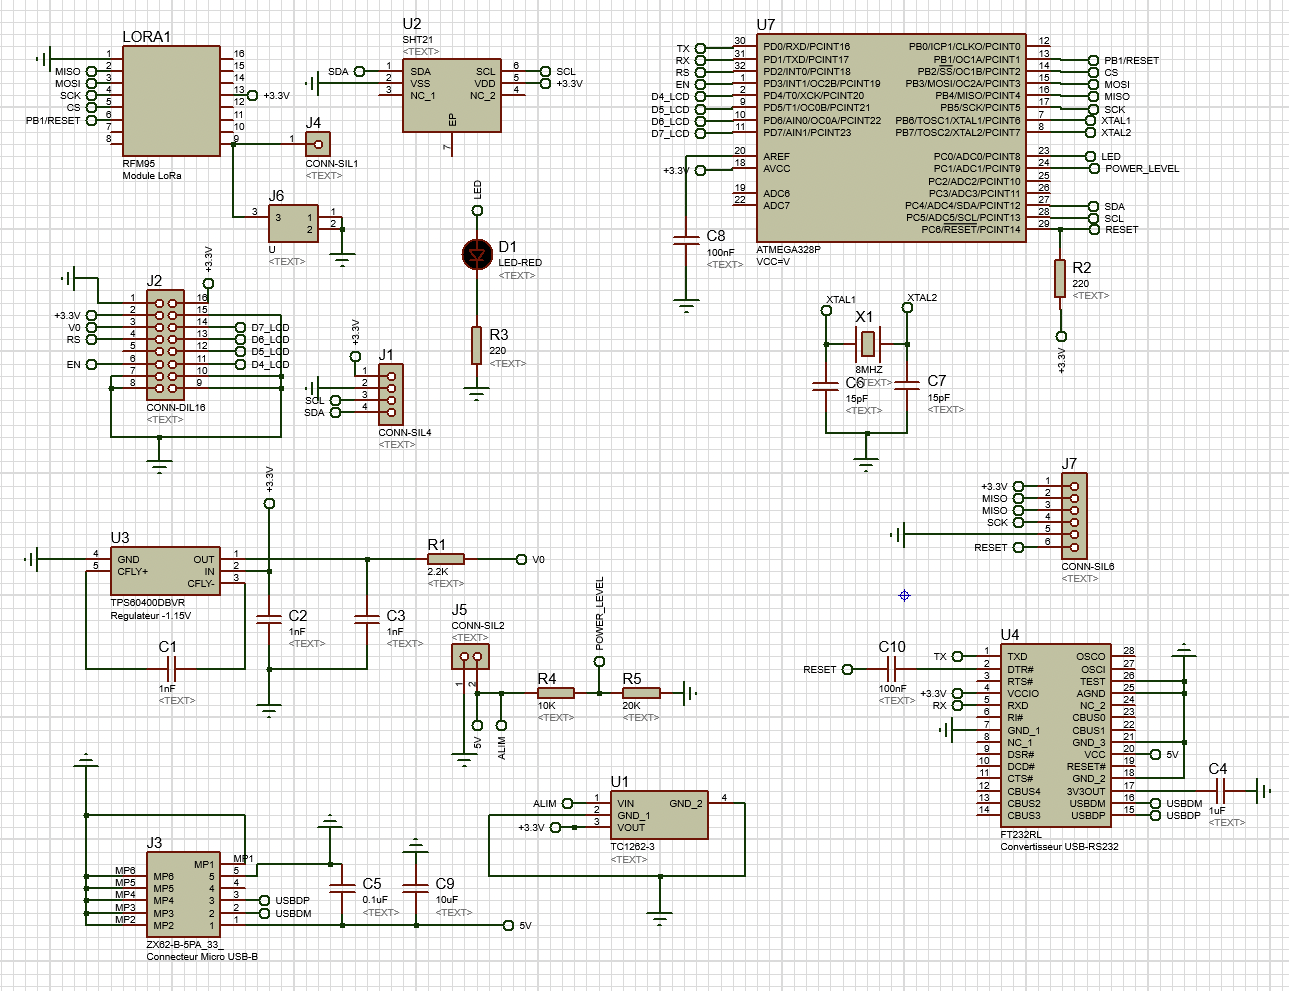
\includegraphics[width=1\textwidth]{img/proteus/schema.png}
                \caption{\label{fig:schema}Schéma de la carte capteur}  
            \end{center}  
        \end{figure}

        Pour la réalisation de la carte capteur, nous avons dans un premier temps récupéré l’ensemble des empreintes des composants. Pour certains, comme le module LORA, il a fallu réaliser son empreinte 
        (schématique et routage) à partir des données de la datasheet. \\
        Une fois les éléments rassemblés sur la feuille du schéma par groupe de fonction (Puissance, capteur, ATMEGA…), nous avons repris les datasheets des différents composants afin de définir les liaisons entre eux.

        

    \clearpage
    \section{Routage}

        \begin{figure}[!h]
            \centering
            \begin{minipage}{.48\linewidth}
                \begin{center}
                    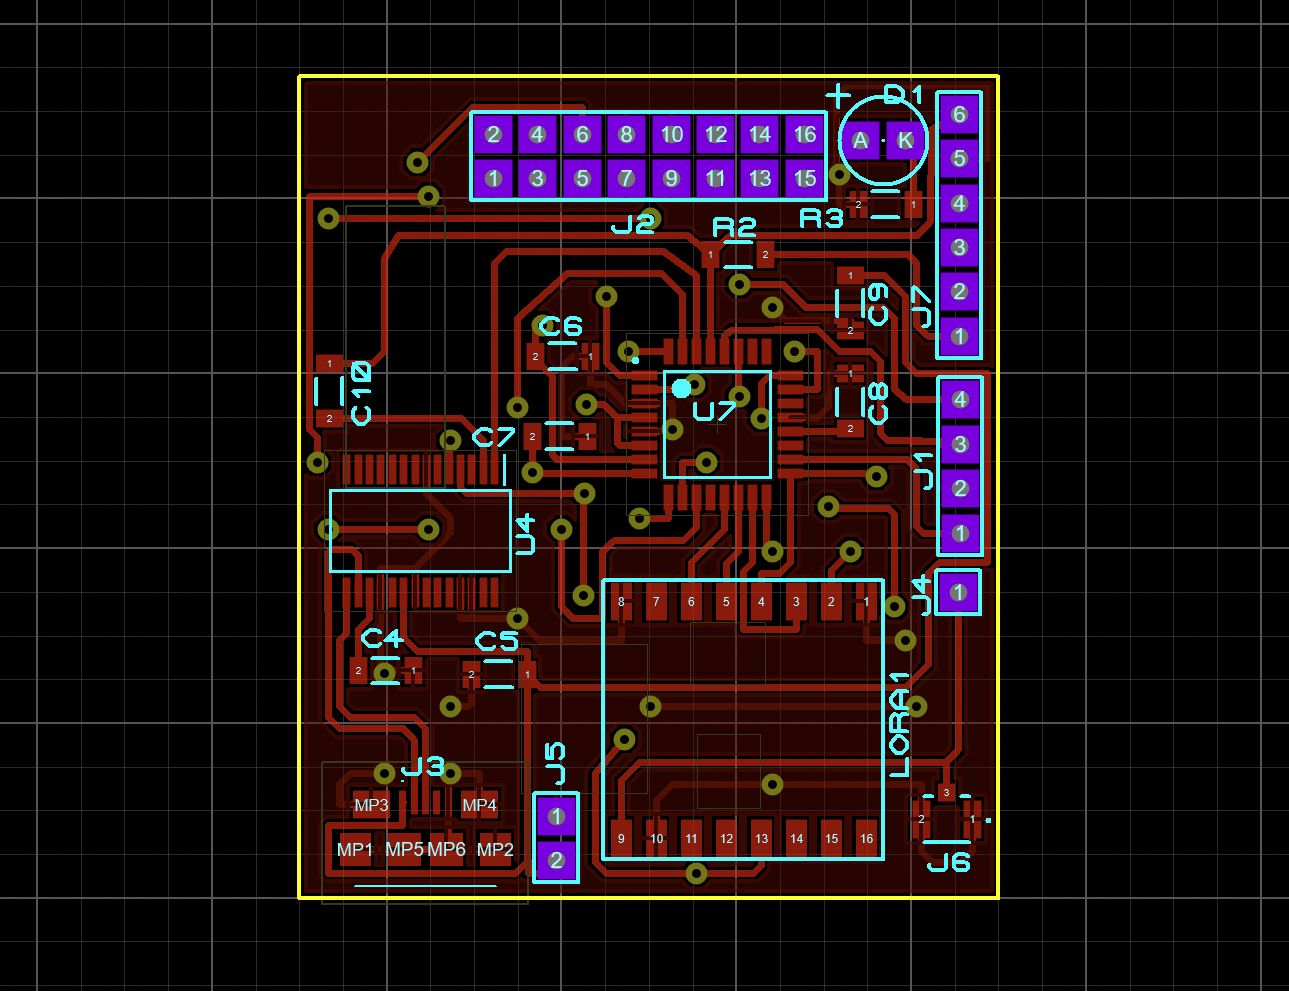
\includegraphics[width=1\textwidth]{img/proteus/routage_top.png}
                    \caption{\label{fig:routage_top}Routage de la carte capteur, couche supérieur}  
                \end{center}
            \end{minipage}\hfill
            \begin{minipage}{.48\linewidth}
                \begin{center}
                    \begin{center}
                        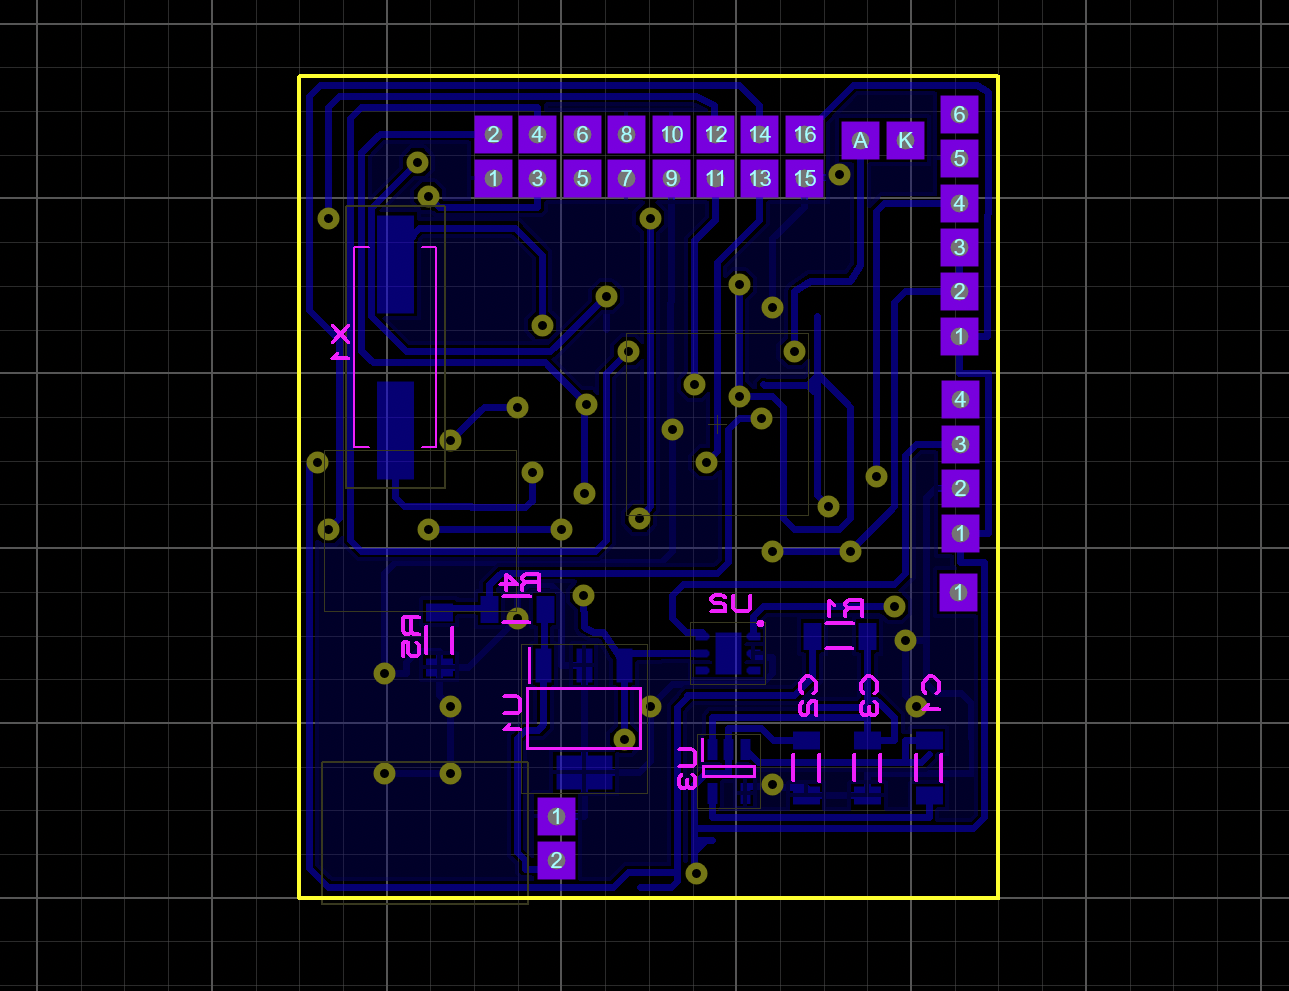
\includegraphics[width=1\textwidth]{img/proteus/routage_bottom.png}
                        \caption{\label{fig:routage_bottom}Routage de la carte capteur, couche inférieur}  
                    \end{center}
                \end{center}
            \end{minipage}
        \end{figure}

        Pour le routage, nous avons fais le choix de grouper nos composants de manière cohérente selon leur fonction. Cela nous a permis de réaliser un routage automatique sans avoir d’erreur. 
        Cependant le routage restait mal optimisé et nous avons donc repris un certain nombre de pistes afin de corriger les angles, limiter le nombre de via et vérifier leur placement sous les composants. \\
        Malheureusement, quelques détails nous ont échappé. L’empreinte du quartz n’était pas la bonne et le placement du LCD n’était pas optimal. Nous avons donc dû recommencer la démarche~: Routage auto/Modification/Vérification.  



    \section{Plan 3D}

        \begin{figure}[!h]
            \centering
            \begin{minipage}{.48\linewidth}
                \begin{center}
                    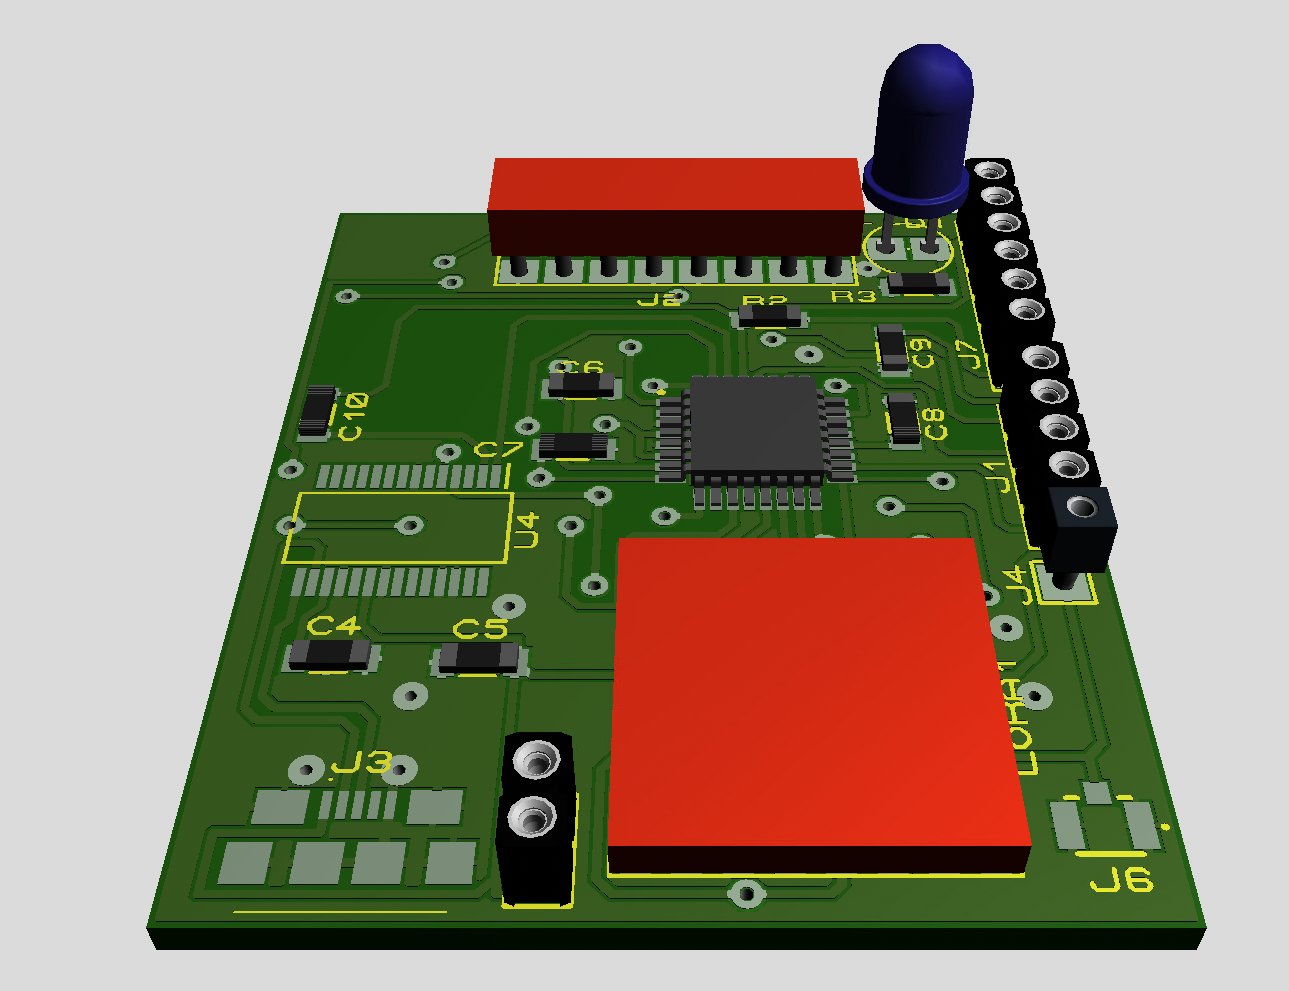
\includegraphics[width=1\textwidth]{img/proteus/3d_top.png}
                    \caption{\label{fig:3d_top}Vue 3D de la carte capteur, couche supérieur}  
                \end{center}
            \end{minipage}\hfill
            \begin{minipage}{.48\linewidth}
                \begin{center}
                    \begin{center}
                        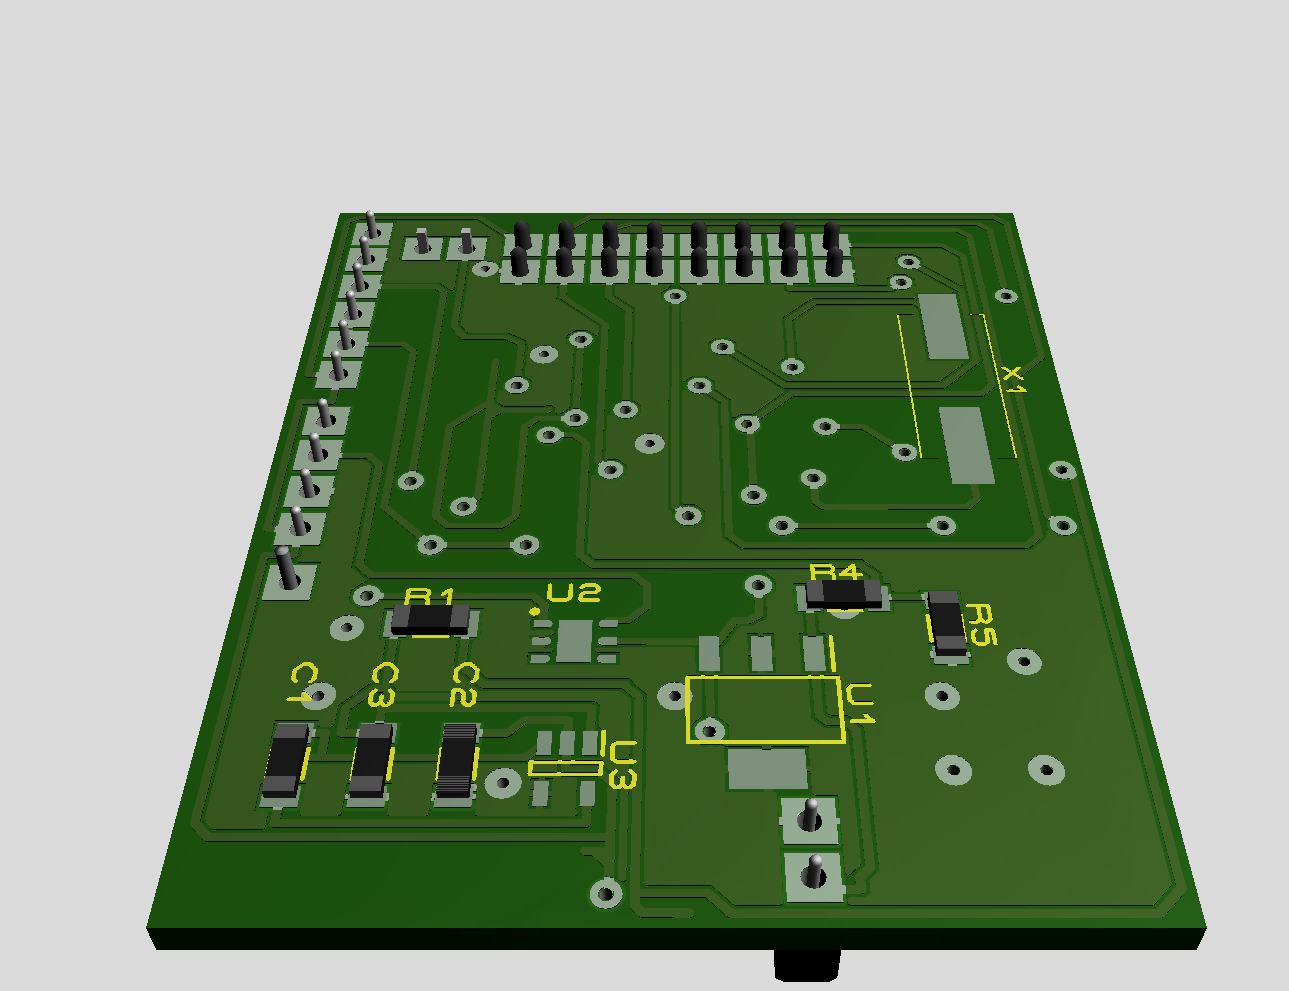
\includegraphics[width=1\textwidth]{img/proteus/3d_bottom.png}
                        \caption{\label{fig:3d_bottom}Vue 3D de la carte capteur, couche inférieur}  
                    \end{center}
                \end{center}
            \end{minipage}
        \end{figure}

\clearpage
\chapter{Codes}
    Nous avons décidé de réaliser les codes dans un projet \textit{PlatformIo} pour des raisons de confort. Le logiciel \textit{Arduino IDE} est très limité, par exemple il n'y a pas d'autocomplétion ou d'indications directes sur des erreurs de syntaxe.
    Alors que sur un projet \textit{PlatformIo} on peut directement utiliser des IDE comme \textit{VSCode} ou encore \textit{CLion} et donc bénéficier de tous leurs avantages. \\
    Cependant, si vous compilez le projet directement, ça ne fonctionnera pas. Il est nécessaire de modifier les \textit{includePath} ou alors recréer le projet et copier les codes qui se trouvent dans le répertoire suivant~:

    \begin{enumerate}
        \item Code de la carte capteur $\to$ \textit{Arduino/code/projet$\_$platformio/sensor$\_$board/src/main.cpp}
        \item Lib de la carte capteur $\to$ \textit{Arduino/code/projet$\_$platformio/sensor$\_$board/lib/...}
        \item Code de la carte serveur $\to$ \textit{ESP$\_$code/projet$\_$platformio/server$\_$board/src/main.cpp}
        \item Lib de la carte serveur $\to$ \textit{ESP$\_$code/projet$\_$platformio/server$\_$board/lib/...}
    \end{enumerate}

    \vspace{0.2 cm}

    \noindent
    Sinon il est également possible d'utiliser nos codes directement dans le logiciel \textit{Arduino IDE} en utilisant les fichiers suivants et en important les librairies au format .zip~:

    \begin{enumerate}
        \item Code de la carte capteur $\to$ \textit{Arduino/code/projet$\_$arduino$\_$ide/main/main.ino}
        \item Lib de la carte capteur $\to$ \textit{Arduino/code/projet$\_$arduino$\_$ide/*.zip}
        \item Code de la carte serveur $\to$ \textit{ESP$\_$code/projet$\_$arduino$\_$ide/main/main.ino}
        \item Lib de la carte serveur $\to$ \textit{ESP$\_$code/projet$\_$arduino$\_$ide/*.zip}
    \end{enumerate}

    \begin{figure}[!h]
        \centering
        \begin{minipage}{.48\linewidth}
            Nous avons également maintenu un dépôt \textit{git} pendant la réalisation des codes, il est disponible en cliquant sur la figure \ref{fig:gitlab}\footnote{Si le lien ne fonctionne pas: \href{https://git.roudaut.xyz}{https://git.roudaut.xyz}}. 
            C'est un serveur GitLab autohéberger, merci de nous prévenir par courriel si vous souhaitez l'utiliser. En tant qu'administrateur, on doit approuver votre demande d'inscription. Sinon, on à laissé le \textit{.git} dans le zip.
        \end{minipage}\hfill
        \begin{minipage}{.48\linewidth}
            \begin{center}
                \begin{center}
                    \href{https://git.roudaut.xyz}{
\includegraphics[width=.8\textwidth]{img/code/GitLab.png}}
                    \caption{\label{fig:gitlab}Lien vers le serveur GitLab}  
                \end{center}
            \end{center}
        \end{minipage}
    \end{figure}








    \section{Carte capteur}
        \subsection{L'architecture du code}
            Pour la mise en œuvre de la carte capteur, nous avons décidé de décomposer le code en plusieurs fichiers comme on peut le voir sur la figure \ref{fig:archi_sensor}. Cela nous permet de garder un code propre sans mélanger les fonctionnalités
            des différents capteurs.

            \clearpage

            \begin{figure}[!h]
                \begin{center}
                    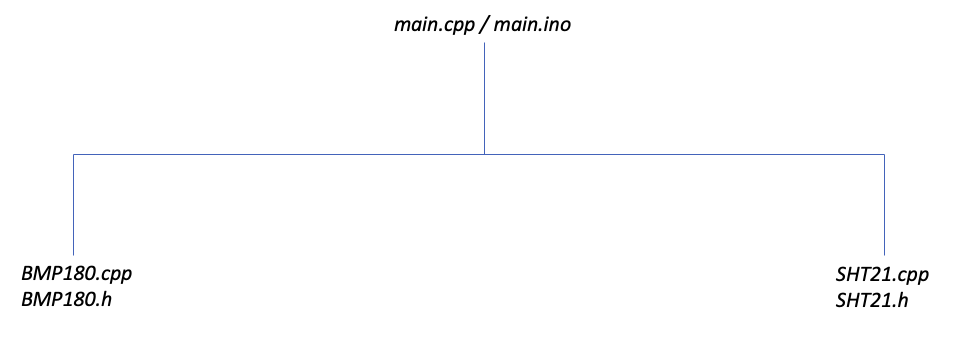
\includegraphics[width=.8\textwidth]{img/code/archi_sensor.png}
                    \caption{\label{fig:archi_sensor}Architecture du code de la carte capteur}  
                \end{center}
            \end{figure}

        \subsection{Programmation du BMP180}
            \noindent
            \subsubsection{Les fonctions}

            \vspace{.2cm}

            Le BMP180 est décomposé en plusieurs fonctions. Les fonctions principales sont publiques et elles permettent d'obtenir la pression et d'initialiser le capteur à partir du \textit{main}. L'initialisation consiste à lire les 
            paramètres de compensations et à initialiser la liaison \textit{I2C}.

\begin{lstlisting}[style=myC, caption=Fonctions publiques de la librairie BMP180, language=C, frame=lines]
long getPressure(); // retourne la pression en long
void begin(); // Lecture des paramètres de compensation
\end{lstlisting}

        \vspace{.5 cm}

        Il y a ensuite les fonctions privées qui permettent d'obtenir la pression brute sur 16~bits ou encore pour convertir cette pression brute en \textit{hPa}. Il n'y a donc aucune utilité pour l'utilisateur de les avoir dans le \textit{main.}

\begin{lstlisting}[style=myC, caption=Fonctions privées de la librairie BMP180, language=C, frame=lines]
int32_t readPressure(); // Lecture de la pression brut
int32_t readTemp(); // Lecture de la temp brut, utile pour le calcul de B5 uniquement
long convertRawPressure(int32_t rawPressure); // Convertion de la pression brut
int32_t read2SignedByte(int8_t addr); // Lecture de 2 octets signés
uint32_t read2UnsignedByte(int8_t addr); // Lecture de 2 octets non signés
\end{lstlisting}

        \vspace{.5 cm}

        L'une des particularités de la \textit{datasheet} que nous n’avions pas très bien compris. C'est qu'il est précisé que la lecture des registres de température et de pression doit être affectée dans des variables de type \textit{short} soit 32~bits. Alors que 
        nous lisons uniquement 16~bits. Nous n'avons pas très bien compris l'utilité, mais comme cela fonctionne nous avons gardé le type \textit{short} pour respecter la \textit{datasheet}.

        \clearpage

        \noindent
        \subsubsection{Algorithme de la lib BMP180}
        \vspace{.2 cm}

        \begin{figure}[!h]
            \begin{center}
                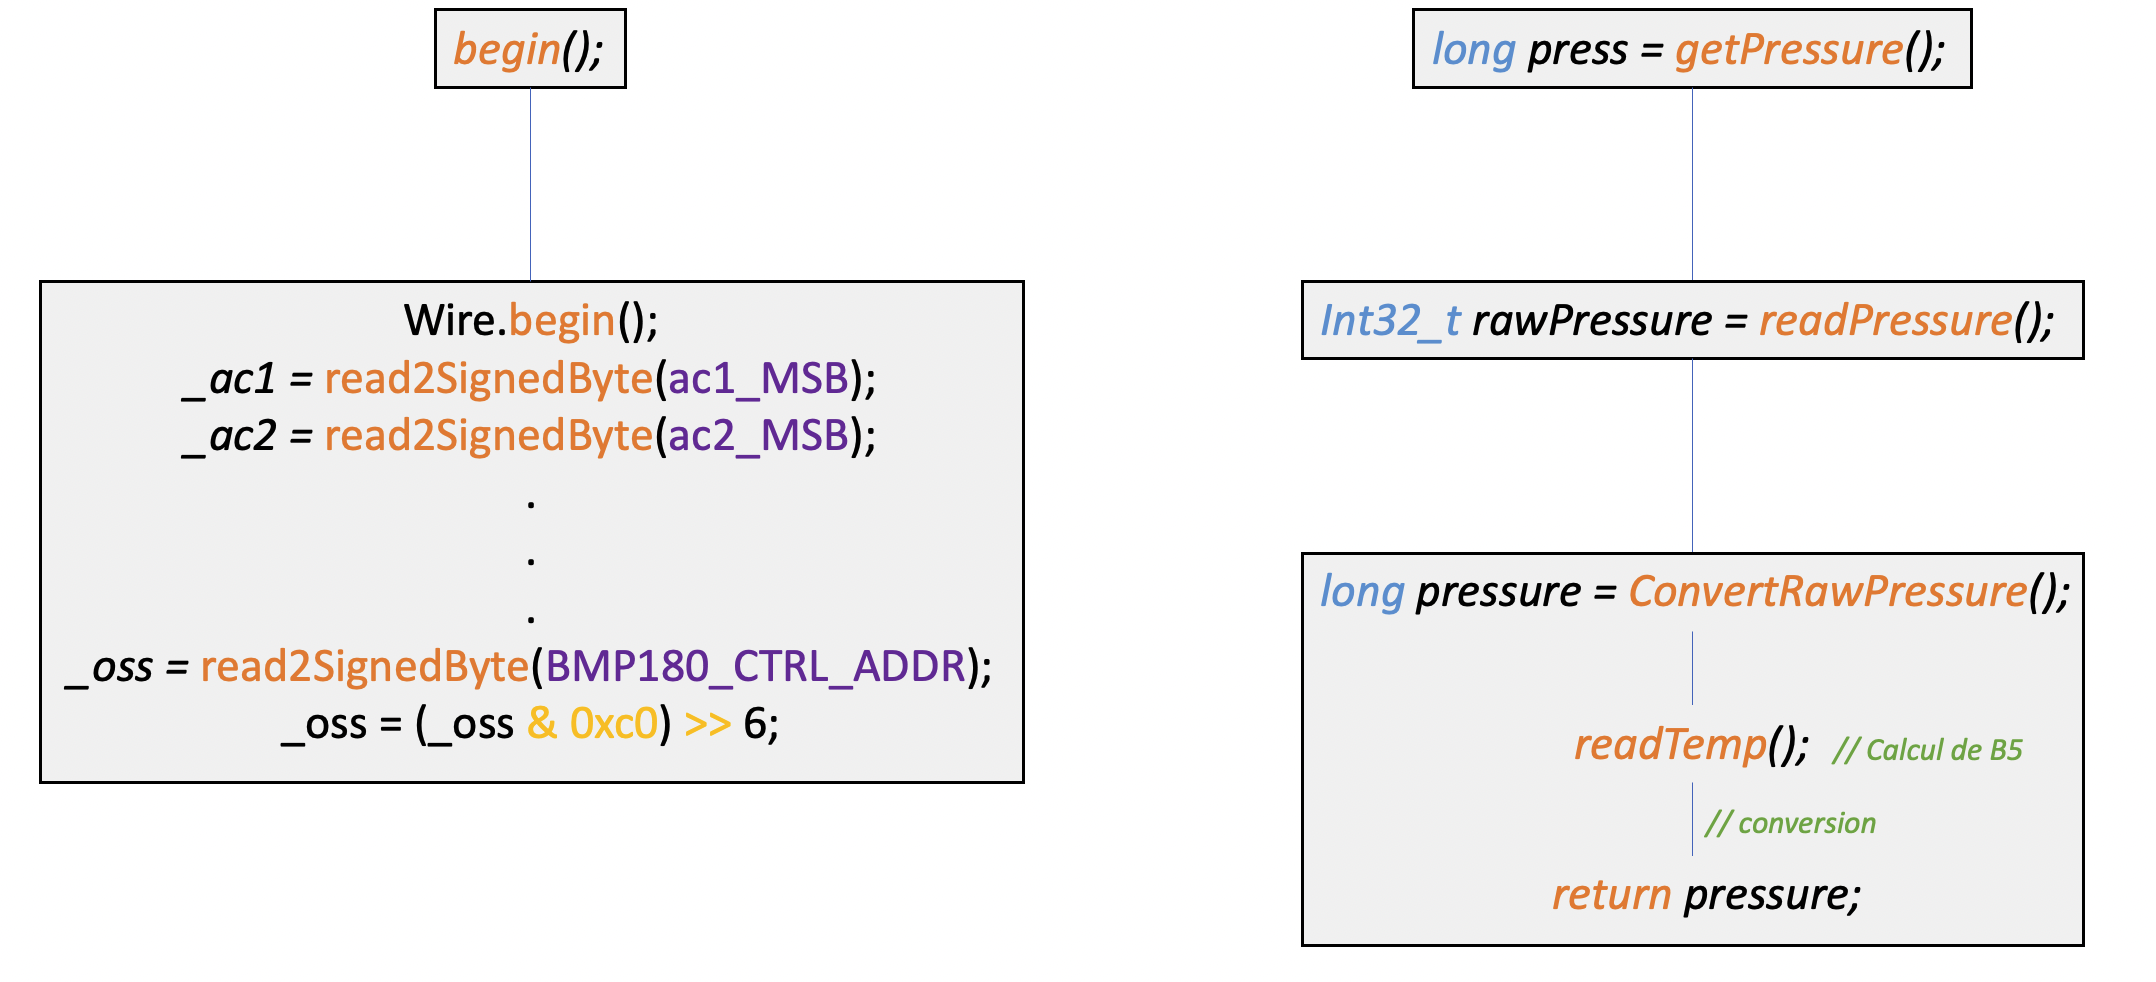
\includegraphics[width=.65\textwidth]{img/code/algo_bmp.png}
                \caption{\label{fig:algo_bmp}Algorithme du BMP180}  
            \end{center}
        \end{figure}

      





        \subsection{Programmation du SHT21}
            \subsubsection{Les fonctions}


            Le SHT21 est décomposé en plusieurs fonctions. Les fonctions principales sont publiques et elles permettent d'obtenir la température, l'humidité et d'initialiser la liaison \textit{I2C} à partir du \textit{main}. 

\begin{lstlisting}[style=myC, caption=Fonctions publiques de la librairie SHT21, language=C, frame=lines]
void begin(); // Initialise la liaison I2C
float getTemp(); // retourne la temp en float
float getRH(); // retourne l'humidité en float
\end{lstlisting}

        \vspace{.5 cm}

        Il y a ensuite les fonctions privées qui permettent d'obtenir la température brute et l'humidité brute sur 16~bits ou encore pour convertir les mesures brutes en valeurs normalisées. Il n'y a donc aucune utilité pour l'utilisateur de les avoir dans le \textit{main.}

\begin{lstlisting}[style=myC, caption=Fonctions privées de la librairie SHT21, language=C, frame=lines]
uint16_t readTemp(); // retourne la temp brut sur 16bits
uint16_t readRH(); // retourne l'humidité brut sur 16bits
float convertRawTemp(uint16_t rawTemp); // Conversion de la temp brut en float
float convertRawRH(uint16_t rawRH); // Conversion de l'humidite brut en float 
\end{lstlisting}

        \subsubsection{Algorithme de la lib SHT21}

        \begin{figure}[!h]
            \begin{center}
                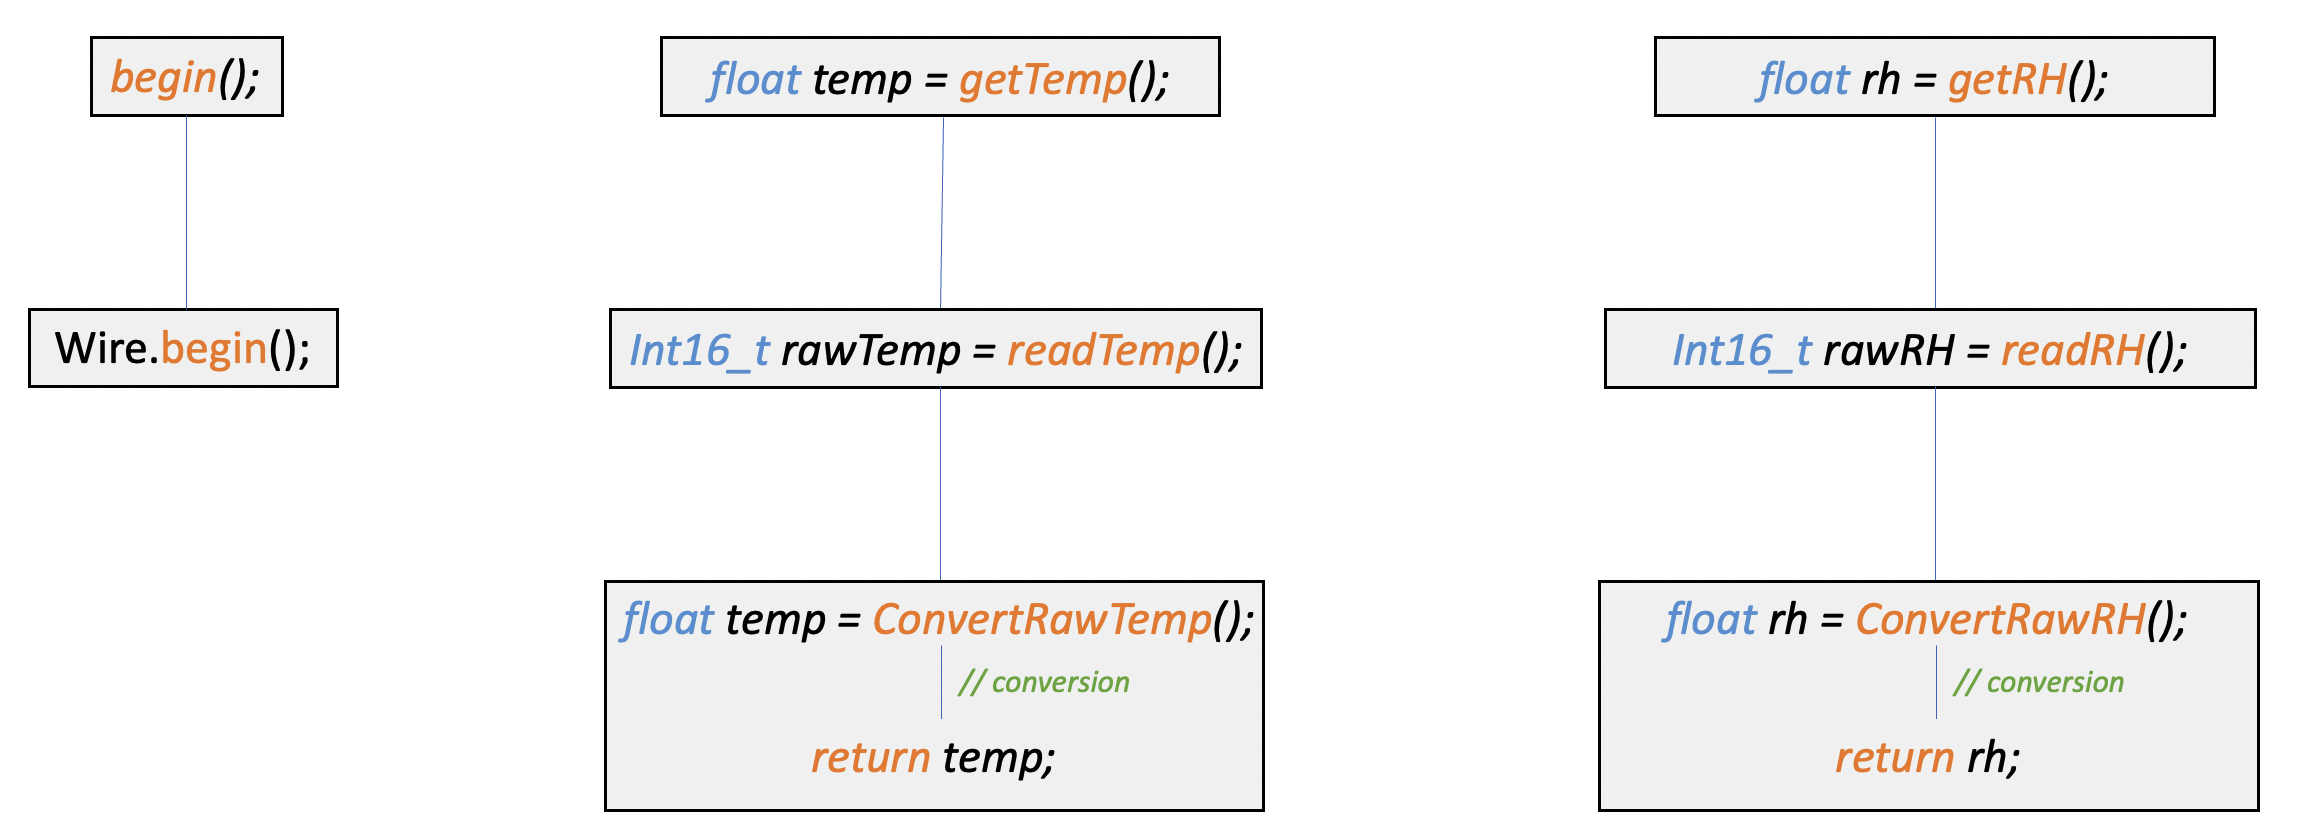
\includegraphics[width=.65\textwidth]{img/code/algo_sht.png}
                \caption{\label{fig:algo_sht}Algorithme du SHT21}  
            \end{center}
        \end{figure}





        \subsection{Mise en œuvre de Lora}
            Nous n'avons pas eu le temps de tester notre code pour la mise en œuvre d'une communication Lora, c'est la raison pour laquelle il est présent, mais commenté pour éviter tous les problèmes. \\
            Comme c'est un code pas très conséquent, nous avons choisi de ne pas réaliser de fichiers séparés et de le mettre directement dans le \textit{main}. \\


\begin{lstlisting}[style=myC, caption=Initialisation de Lora pour la carte capteur, language=C, frame=lines]
SPI.begin(); // intialisation des pins
LoRa.setPins(); // intialisation des pins

unsigned int myDelay = millis();

int ret = 0;
while ((myDelay + 10000) > millis()){ // delai de 10sec pour établir la communication Lora
    ret = LoRa.begin(LORA_FREQUENCY);

    if (ret){
    Serial.println("Starting LoRa success!");
    LoRa.setSyncWord(0xa2);
    break;
    }
}

if (!ret){ // gestion d'err
    Serial.println("Starting LoRa failed!");
}
\end{lstlisting}

\begin{lstlisting}[style=myC, caption=Emission de données, language=C, frame=lines]
void loraSendData(float temp, float rh, long press)
{
    LoRa.beginPacket();
    LoRa.print(temp);
    LoRa.print(rh);
    LoRa.print(press);
    LoRa.endPacket();
}
\end{lstlisting}



        \subsection{Le programme principal (main)}
            Le \textit{main} est comme son nom l'indique le fichier principal de notre code. En déclarant des objets liés aux classes des librairies précédemment décrites, nous allons pouvoir afficher les différentes mesures. \\

            \noindent
            Il faut dans un premier temps inclure nos librairies puis déclarer les objets~:

\begin{lstlisting}[style=myC, caption=Ajout des librairies et déclaration des objets, language=C, frame=lines]
// Librairies de base de arduino
#include <Arduino.h>
#include <LiquidCrystal.h>
#include <Wire.h>
#include <LoRa.h>

// Librairies faites par nous-meme pour utiliser les capteurs de la carte serveur
#include <sht21.h>
#include <bmp180.h>

// Declaration des objets des classes
LiquidCrystal lcd(rs, en, d4, d5, d6, d7);
BMP180 bmp;
SHT21 sht;
\end{lstlisting}

            \vspace{.5 cm}  

            \noindent
            Initialisation des différents capteurs et du wifi~: 


\begin{lstlisting}[style=myC, caption=Initialisation, language=C, frame=lines]
lcd.begin(16, 2);
bmp.begin();
sht.begin();
Serial.begin(9600);
\end{lstlisting}

            \vspace{.5 cm}

            \noindent
            Suite à ces déclarations, on peut utiliser les objets pour obtenir les différentes mesures~: 

\begin{lstlisting}[style=myC, caption=Lecture de température sur le SHT21, language=C, frame=lines]
float temp = sht.getTemp();
\end{lstlisting}

            \vspace{.5 cm}
            Comme on peut le constater avec cet exemple. Le choix d'avoir fait une classe par capteur, nous permet de structurer plus facilement notre code et de garder code un propre et facile à comprendre.\\

            \subsubsection{Algorithme de notre code}

                \begin{figure}[!h]
                    \begin{center}
                        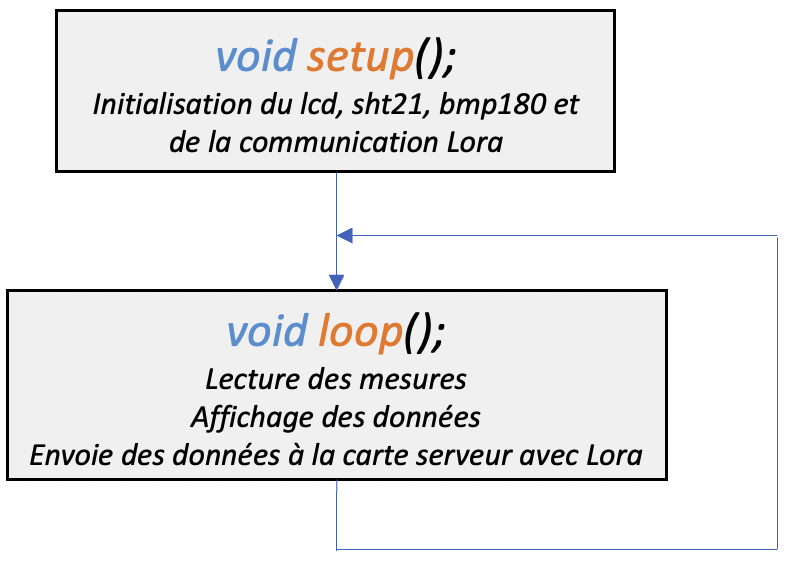
\includegraphics[width=.4\textwidth]{img/code/algo_main_sensor.png}
                        \caption{\label{fig:algo_main_sensor}Algorithme du main de la carte capteur}  
                    \end{center}
                \end{figure}




        \subsection{Simulation et test sur carte}
            \subsubsection{Simulation}

                \begin{figure}[!h]
                    \centering
                    \begin{minipage}{.48\linewidth}
                        Comme nous pouvons le constater sur la figure \ref{fig:simu_sensor}, la première ligne correspond aux valeurs du \textit{SHT21} et la seconde aux valeurs du \textit{BMP180}. Les mesures de la première ligne sont cohérentes, mais pas sur la seconde. 
                        La température est bonne contrairement à la pression. Plusieurs de nos camarades avaient également ce problème, il est donc possible de se demander si l'erreur ne viendrait pas de la simulation plutôt que de notre code.
                    \end{minipage}\hfill
                    \begin{minipage}{.48\linewidth}
                        \begin{center}
                            \begin{center}
                                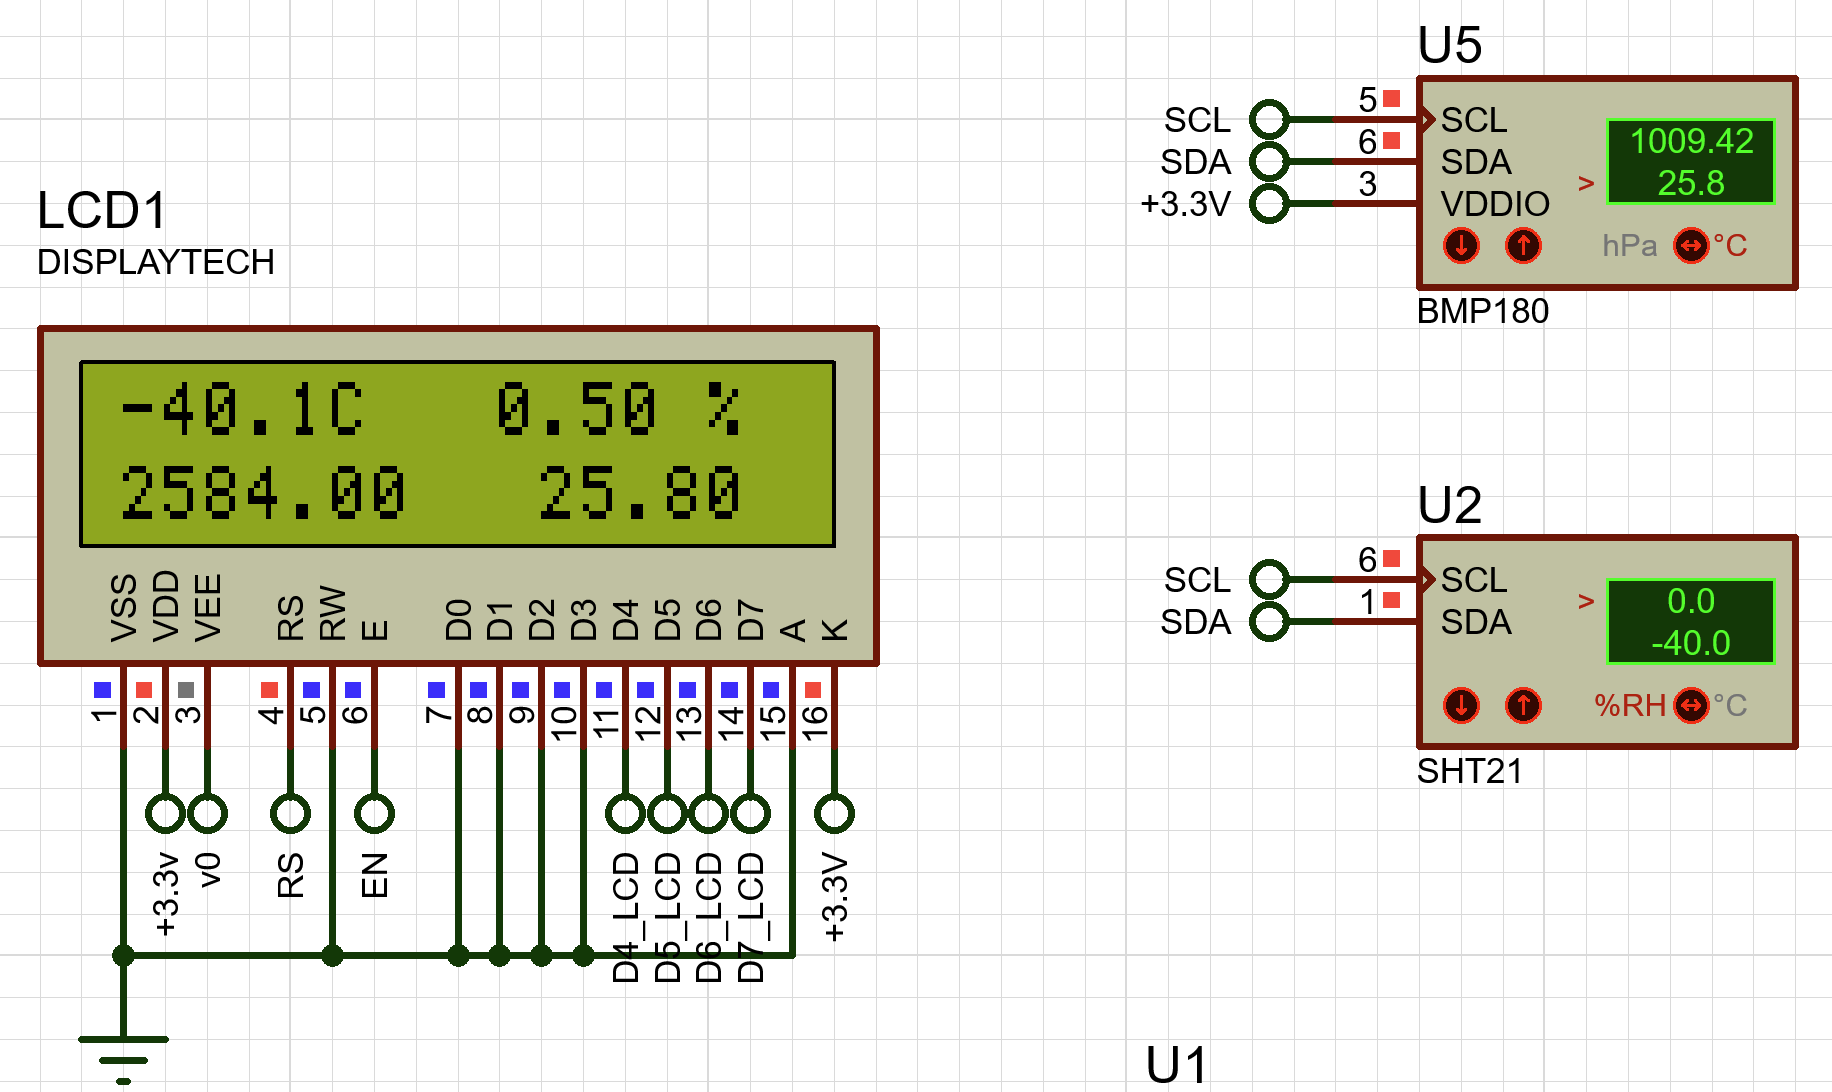
\includegraphics[width=1\textwidth]{img/code/simu_sensor.png}
                                \caption{\label{fig:simu_sensor}Simulation de la carte capteur}  
                            \end{center}
                        \end{center}
                    \end{minipage}
                \end{figure}
            


            \subsubsection{Tests sur carte}
                Maintenant que le programme de la carte capteur terminé, il est nécessaire de le téléverser sur cible. Pour cela, il faut dans un premier temps implémenter un bootloader. Il permet de téléverser et exécuter nos programmes arduino. Lors de son implémentation, nous nous sommes rendu compte d’une erreur sur le schéma. Le connecteur~J7 du 
                bootloader est connecté à deux pins MISO au lieu de 1~pin MISO et 1~pin MOSI.  \\

                \noindent
                Pour charger le bootloader il a donc fallu couper une piste et ressouder des fils~:
                
                \begin{enumerate}
                    \item Entre le Pin~2 du J7 et 3 du module LORA  
                    \item Entre le Pin~3 du J7 et 2 du module LORA \\
                \end{enumerate}

                Ensuite, nous avons téléversé un premier code de test qui fait simplement clignoter la LED de la carte capteur. L’exécution est correcte, nous pouvons donc téléverser le programme principal. Mais le programme ne se téléverse pas.
                Nous avons alors essayé de comprendre le problème en procédant par élimination. \\
                Vérifier dans un premier temps le code. Pour cela, nous l’avons téléversé sur une autre carte capteur de nos camarades. Le programme se téléverse bien sur leur carte, mais toujours pas sur la nôtre. 
                De même, le code pour faire clignoter la LED ne se téléverse pas non plus. Ce n’est donc pas un problème d’ordinateur, de compilation ou de câble et port USB. \\
                Le problème logiciel semblait écarté. Nous avons donc vérifié la carte en passant celle-ci au peigne fin de la loupe, mais aucune trace de cours circuits. En vérifiant les tensions de la carte, l’ensemble des composants étaient correctement alimentés. \\

                À ce stade-là, nous étions quasi certains d’avoir un code bon et une carte fonctionnelle. Puisque c’est le bootloader qui permet de charger le programme et que c’est justement ce que nous n’arrivons pas à faire, nous avons décidé de recharger le bootloader avec monsieur BERTHOLOM. \\
                Après plusieurs tentatives échouées suite à un mauvais câblage et différents tests effectués, nous avons finalement réussi à recharger le bootloader. Le test du code pour faire clignoter la LED fonctionne, mais en voulant téléverser notre programme principal, ECHEC. 
                Une nouvelle fois, nous avons pu charger un programme puis plus aucun. Nous avons alors émis l’hypothèse que le programme venait écraser le bootloader et que celui-ci ne pouvait donc plus charger de nouveaux programmes. \\
                Les manipulations ont été refaites plusieurs fois afin de vérifier les vitesses de transmission, les signatures et enfin d’étudier les messages d’erreurs. Nous avons pu mettre en lumière plusieurs points comme le changement de signature selon la tension +3,3~V et +5~V.
                Grâce à ses tests, monsieur BERTHOLOM a fait un fichier avec l’ensemble des erreurs recensées. \\

                Par manque de temps pour plus d’investigations, nous sommes donc arrêtés au point de pouvoir téléverser une seule fois notre programme. Comme le module LORA nécessite d’être soudé après le chargement du bootloader, nous n’avons pas pu vérifier notre code avec la fonction de transmission LORA.  





    \section{Carte serveur}
        \subsection{L'architecture du code}
            Pour la mise en œuvre de la carte serveur, nous avons décidé de décomposer le code en plusieurs fichiers comme on peut le voir sur la figure \ref{fig:archi_server}. Cela nous permet de garder un code propre sans mélanger les fonctionnalités
            des différents capteurs.


            \clearpage
            \begin{figure}[!h]
                \begin{center}
                    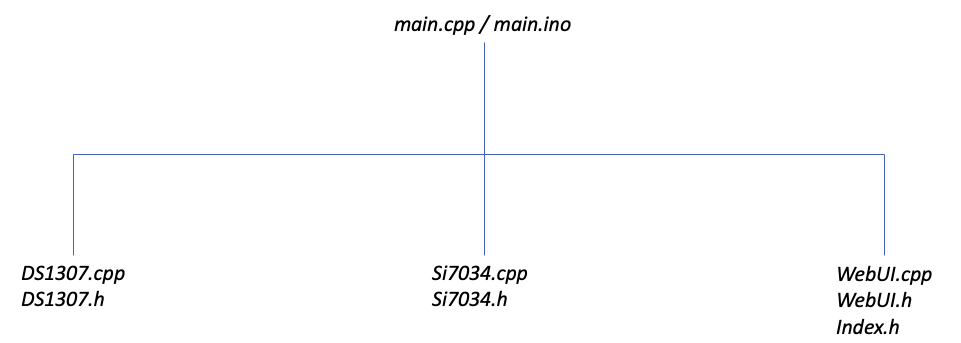
\includegraphics[width=.8\textwidth]{img/code/archi_server.png}
                    \caption{\label{fig:archi_server}Architecture du code de la carte serveur}  
                \end{center}
            \end{figure}





        \subsection{Programmation du DS1307}
            \subsubsection{Les fonctions}


            Le \textit{DS1307} est décomposé en plusieurs fonctions. Les fonctions principales sont publiques et elles permettent de configurer l'heure actuelle grâce à un serveur ntp
            et la seconde permet d'obtenir l'heure du \textit{DS1307}.

\begin{lstlisting}[style=myC, caption=Fonctions publiques de la librairie DS1307, language=C, frame=lines]
void begin(); // Initialise la liaison I2C
void setupRealTime(struct tm *time); // Configuration à partir du serveur ntp 
void getRealTime(struct MyTime *myTm); // Retourne une structure avec l'heure du RTC
\end{lstlisting}

        \vspace{.5 cm}

        Il y a ensuite les fonctions privées qui permettent de convertir un \textit{BCD} en décimal et inversement. Il n'y a donc aucune utilité pour l'utilisateur de les avoir dans le \textit{main.}

\begin{lstlisting}[style=myC, caption=Fonctions privées de la librairie DS1307, language=C, frame=lines]
uint8_t decToBcd(uint8_t dec); // conversion decimal a bcd
uint8_t bcdToDec(uint8_t bcd); // conversion bcd a decimal
int actualYear(int yearsFrom1900); // conversion du temps ecoule depuis 1900
\end{lstlisting}


        \subsubsection{Le fonctionnement}

        Dans un premier temps, il est nécessaire de configurer le wifi avec un \textit{ssid} et un \textit{password} définis au préalable. De nombreux exemples existent sur internet, celui-ci en fait partie~:

\begin{lstlisting}[style=myC, caption=Initialisation du wifi dans le main, language=C, frame=lines]
WiFi.begin(ssid, password);
while(WiFi.waitForConnectResult() != WL_CONNECTED){      
    Serial.print(".");
}
Serial.println("");
Serial.print("Connected to ");
Serial.println(ssid);
Serial.print("IP address: ");
Serial.println(WiFi.localIP());  
\end{lstlisting}

        \vspace{.2 cm}
        \noindent
        Pour configurer le \textit{DS1307} il faut procéder en plusieurs étapes~:
        \begin{enumerate}
            \item Synchronisation de l'ESP avec l'heure NTP, fonction \textit{configTime()} de \textit{esp32-hal-time.c}.
            \item Déclaration d'une instance de la structure \textit{struct tm} déclaré dans lib \textit{Time.h} de arduino.
            \item Obtention de l'heure actuelle avec \textit{getLocalTime()} de \textit{esp32-hal-time.c}, cette fonction doit prendre en paramètre l'adresse de l'instance de la structure \textit{tm} précédemment créer pour que ses valeurs puissent être modifiées. 
            \item Configuration du \textit{DS1307} avec notre fonction \textit{setupRealTime} située dans \textit{DS1307.h}, cette fonction doit également prendre l'adresse de notre instance de la structure \textit{tm} pour que ses valeurs puissent être utilisées.
        \end{enumerate}

        \vspace{.5 cm}

        \noindent
        \textsc{Exemple~:}
        
\begin{lstlisting}[style=myC, caption=Configuration du DS1307, language=C, frame=lines]
DS1307 clk;

configTime(0, 3600, ntpServer); // configuration du temps réel sur l'esp
                                // depuis le serveur ntp
struct tm rtm; // Structure déclaré dans la lib time.h de arduino

if(getLocalTime(&rtm)){ // retourne l'heure du esp32 configuré avec le ntp
    clk.setupRealTime(&rtm); // configuration du DS1307
}
\end{lstlisting}

        \vspace{.5 cm}

        \noindent
        Pour lire l'heure du \textit{DS1307} il faut également procéder en plusieurs étapes~:
        \begin{enumerate}
            \item Déclaration d'une instance de la structure \textit{struct MyTime} déclarée dans notre lib \textit{DS1307.h}.
            \item Appel de notre fonction \textit{getRealTime()}, avec en paramètre l'adresse de l'instance de la structure \textit{MyTime} précédemment créée pour que ses valeurs puissent être modifiées.
            \item Utilisation de l'instance de la structure \textit{MyTime} pour lire les valeurs du \textit{DS1307}.
        \end{enumerate}

        \vspace{.2cm}

        \noindent
        Le fait que notre fonction a comme paramètre un pointeur permet de modifier directement les valeurs de l'implémentation de notre structure sans avoir besoin de créer une nouvelle à chaque fois ou de retourner une structure. Cela permet une économie de mémoire et de performance. Deplus il est beaucoup plus pratique d'utiliser une structure quand on a autant de données à retourner, contrairement
        capteur de température et d'humidité.

        \vspace{.5 cm}

        \noindent
        \textsc{Exemple~:}

\begin{lstlisting}[style=myC, caption=Lire l'heure du DS1307, language=C, frame=lines]
DS1307 clk;

struct MyTime myTime;
clk.getRealTime(&myTime);
int secondes = myTime.secondes;
\end{lstlisting}


        \vspace{.5cm}

        Pour une meilleure compréhension du pourquoi, on doit donner en paramètre l'adresse de notre structure. C'est dû au fait que dans notre fonction \textit{getRealTime} on affecte directement à nos différentes variables de la structure les valeurs du \textit{DS1307}~: \\
        
        \noindent
        \textsc{Exemple~:} \textit{(Extrait de notre fonction, elle n'est pas complète ici~!)}

\begin{lstlisting}[style=myC, caption=Extrait de la fonction getRealTime,  language=C, frame=lines]
void DS1307::getRealTime(struct MyTime *myTm){
    // Wire.beginTran [...]
    myTm -> month = bcdToDec(Wire.read());
    // [...]
}
\end{lstlisting}







        \subsection{Programmation du Si7034}
            \subsubsection{Les fonctions}


            Le \textit{Si7034} est décomposé en plusieurs fonctions. Les fonctions principales sont publiques et elles permettent d'obtenir la température, l'humidité et d'initialiser la liaison \textit{I2C} à partir du \textit{main}.

\begin{lstlisting}[style=myC, caption=Fonctions publiques de la librairie Si7034, language=C, frame=lines]
void begin(); // Initialisation de la liaison I2C
float getTemp(); // Retourne la température en float
float getRH(); // Retourne l'humidité en float
\end{lstlisting}

        \vspace{.5 cm}

        Il y a ensuite les fonctions privées qui permettent d'obtenir la température brute et l'humidité brute sur 16~bits ou encore pour convertir les mesures brutes en valeurs normalisées. Il n'y a donc aucune utilité pour l'utilisateur de les avoir dans le \textit{main.}

\begin{lstlisting}[style=myC, caption=Fonctions privées de la librairie Si7034, language=C, frame=lines]
uint16_t readRawTemp(); // retourne la temp brut sur 16bits
uint16_t readRawRh(); // retourne l'humidité brut sur 16bits
float convertRawTemp(uint16_t rawTemp); // conversion de la temp brut en float
float convertRawRH(uint16_t rawRH); // conversion de l'humidité brut en float 
\end{lstlisting}


        \subsubsection{Algorithme de la lib Si7034}

        \begin{figure}[!h]
            \begin{center}
                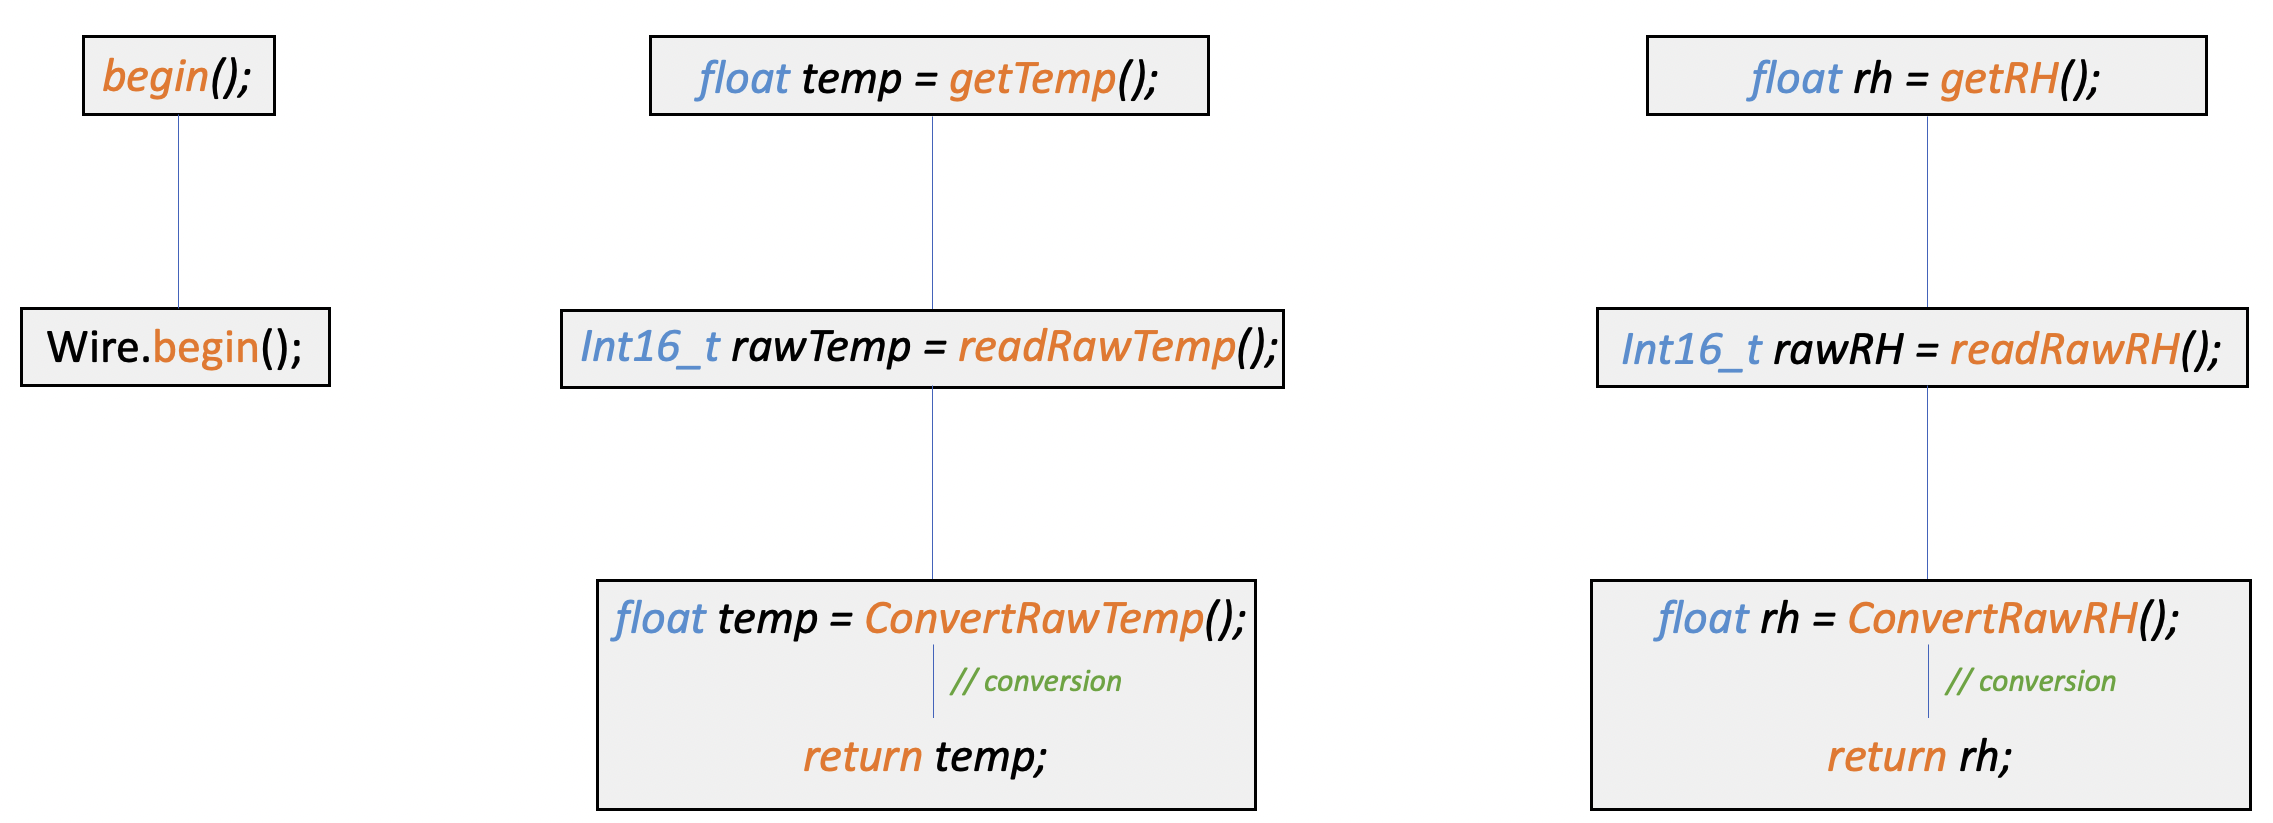
\includegraphics[width=.7\textwidth]{img/code/algo_si.png}
                \caption{\label{fig:algo_si}Algorithme du Si7034}  
            \end{center}
        \end{figure}


        \subsubsection{Problèmes rencontrés}    
        dans la \textit{datasheet} il est précisé que la trame pour une lecture des registres de mesure doit ce comporter de la manière suivante~: \\
        
        \begin{figure}[!h]
            \begin{center}
                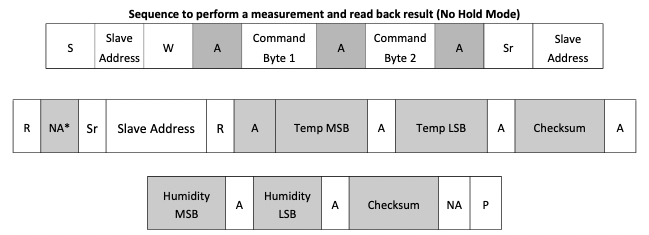
\includegraphics[width=0.6\textwidth]{img/code/fake_trame_si.png}
                \caption{\label{fig:fake_trame_si}Trame de transmission du Si7034 dans la datasheet}  
            \end{center}
        \end{figure}

        \noindent
        En respectant cette trame, la mesure des capteurs n’a pas fonctionné. Après plusieurs recherches, nous avons trouvé un site internet, expliquant la lecture de mesure d'une manière différente qui fonctionne. C'est pourquoi nous l'avons utilisé et que notre 
        code ne correspond pas totalement à la trame de la \textit{datasheet}. Cette méthode consiste à lire les registres du capteur en deux fois plutôt qu'une. \\

        \begin{figure}[!h]
            \begin{center}
                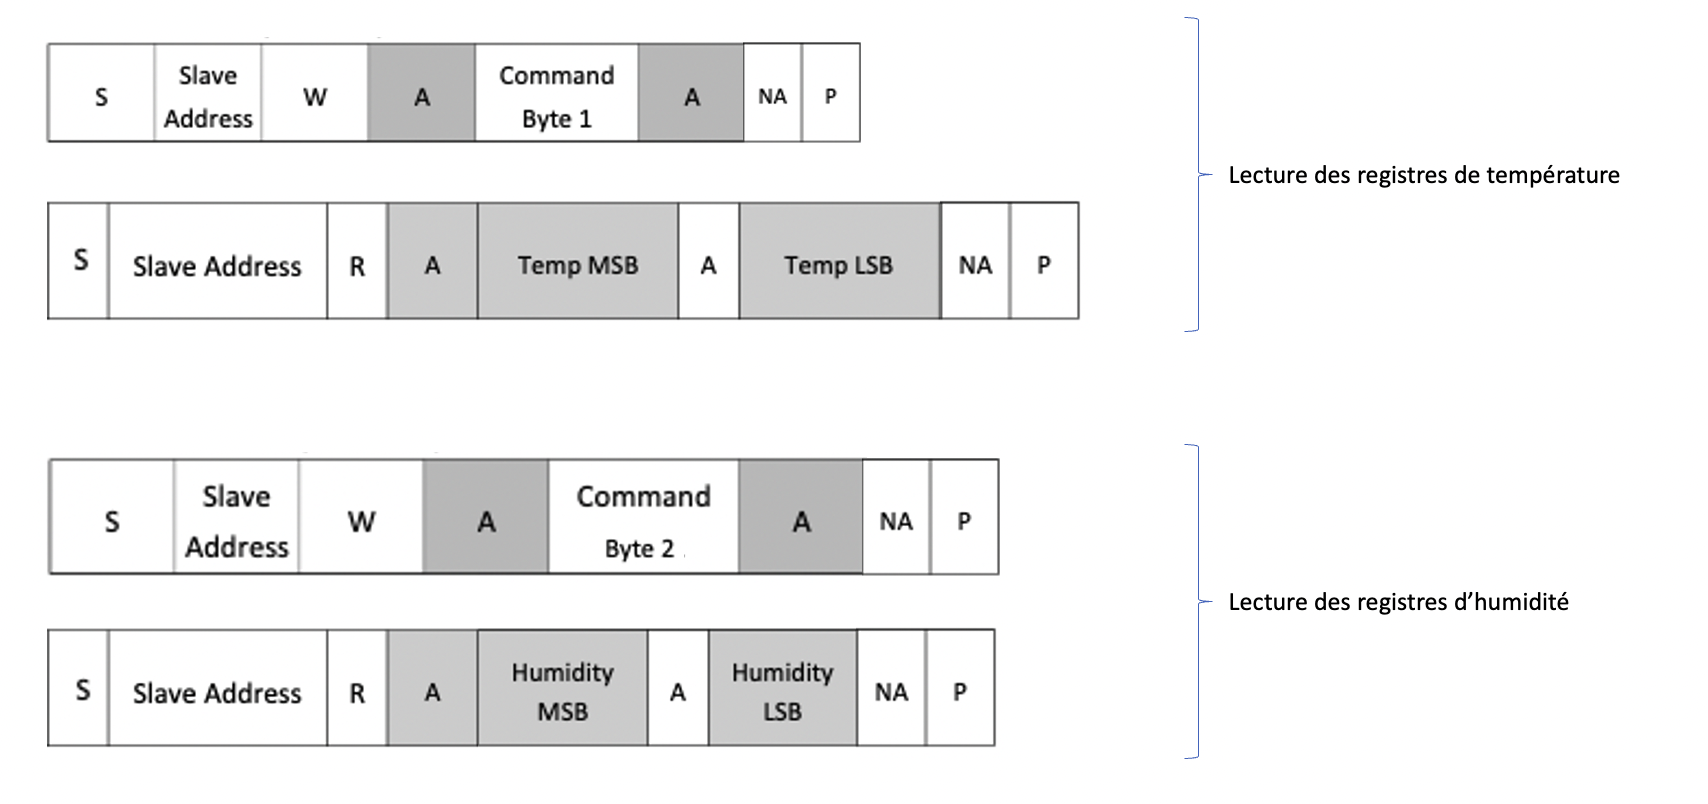
\includegraphics[width=0.8\textwidth]{img/code/trame_si.png}
                \caption{\label{fig:trame_si}Trame de transmission utilisée pour le Si7034}  
            \end{center}
        \end{figure}





        \subsection{Mise en œuvre de Lora}
            Nous n'avons pas eu le temps de tester notre code pour la mise en œuvre d'une communication Lora, c'est la raison pour laquelle il est présent, mais commenté pour éviter tous les problèmes. \\
            Comme c'est un code pas très conséquent, nous avons décidé de ne pas réaliser de fichiers séparés et de le mettre directement dans le \textit{main}.

\begin{lstlisting}[style=myC, caption=Initialisation de Lora pour la carte serveur, language=C, frame=lines]
SPI.begin(SCK, MISO, MOSI, SS); // intialisation des pins
LoRa.setPins(SS, RESET, DIO0); // initialisation des pins

int myDelay = millis();

int ret = 0;
while ((myDelay + 10000) > millis()){ // delai de 10sec pour établir la communication Lora
    ret = LoRa.begin(LORA_FREQUENCY);

    if (ret){
    Serial.println("Starting LoRa success!");
    LoRa.setSyncWord(0xa2);
    break;
    }
}

if (!ret){ // gestion d'err
Serial.println("Starting LoRa failed!");
}
\end{lstlisting}

\begin{lstlisting}[style=myC, caption=Réception de données, language=C, frame=lines]
void loraGetData(){
    int packetSize = LoRa.parsePacket();
    
    // Si des paquets sont à lire alors on les lis
    if (packetSize) {
        while (LoRa.available()) {
        outTemperature = LoRa.read();
        outHumidity = LoRa.read();
        outPressure = LoRa.read();
        }
    }
}
\end{lstlisting}


        \subsection{Mise en œuvre du serveur Web}

            \begin{figure}[!h]
                \begin{center}
                    \includegraphics[width=.9\textwidth]{img/code/webUI.png}
                    \caption{\label{fig:WebUI}Rendu de notre interface web}  
                \end{center}
            \end{figure}

            Le rendu final de notre interface web, figure \ref{fig:WebUI}, intègre les valeurs réelles du \textit{SI7034} et \textit{DS1307}. Nous n’avons pas pu tester notre code Lora comme expliqué plus tôt, les mesures extérieures sont donc de fausses valeurs.\\


            \subsubsection{Les fonctions}

                \noindent
                L'interface web qui porte comme nom de classe \textit{WEBUI} est décomposée en plusieurs fonctions~:

\begin{lstlisting}[style=myC, caption=Fonctions publiques de WEBUI, language=C, frame=lines]
void begin(); // Initialisation du serveur web et des événements pour les requettes AJAX
void displayValue(); // affichage des valeurs sur l'interface web
// Configuration des valeurs pour les afficher sur l'interface :
void setValue(float *inTemp, float *inRh, float *outTemp, float *outRh, long *Press, struct MyTime *myTm);
\end{lstlisting}

                \vspace{.5 cm}

                \noindent
                Il y a ensuite les fonctions qui permettent de réaliser les événements des requêtes \textit{AJAX}\footnote{Asynchronous JavaScript and XML} qui sont en lien avec le serveur web et l'interface web pour permettre l'affichage des données~:

\begin{lstlisting}[style=myC, caption=Fonctions pour les évenements, language=C, frame=lines]
void handleRoot(); // Permet l'affichage de la page principale
void handleInTemp(); // Permet l'affichage de la temp intérieur
void handleInRh(); // Permet l'affichage de l'humidité intérieur
void handleOutTemp();
void handleOutRh();
void handlePress();
void handleDay();
void handleMonth();
void handleYear();
void handleHour();
void handleMin();
void handleSec();
\end{lstlisting}


            \subsubsection{Le fonctionnement}

                \begin{figure}[!h]
                    \begin{center}
                        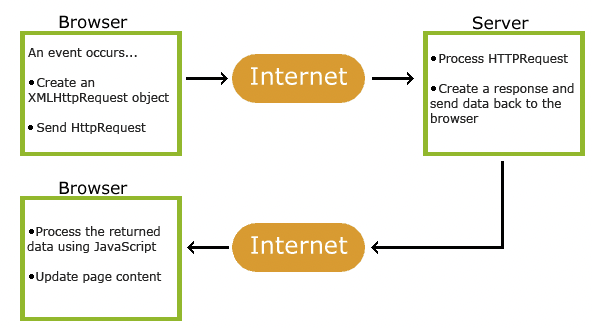
\includegraphics[width=0.7\textwidth]{img/code/AJAX.png}
                        \caption{\label{fig:AJAX}Fonctionnement d'AJAX}  
                    \end{center}
                \end{figure}

                La figure \ref{fig:AJAX}, décrit parfaitement le fonctionnement du protocole \textit{AJAX}. Notre interface web va envoyer des requêtes de lecture au serveur à un certain intervalle, puis le serveur va répondre avec une requête d'écriture au 
                site web. Ensuite, l'interface web va s'occuper de réceptionner les valeurs puis de les afficher. \\
                
                \vspace{.5 cm}

                \noindent
                \textsc{Exemple avec la température~:}

                \vspace{.2 cm}
                
                Dans un premier temps, il faut créer l'événement et indiquer quelle fonction qu’il doit réaliser lorsqu'il arrive. Si le serveur reçoit une requête avec pour \textit{id~: readIndoorTemp}, il devra réaliser la fonction \textit{handleInTemp()}~: 

\begin{lstlisting}[style=myC, caption=Requête réalisée par l'interface web, language=C, frame=lines]
server.on("/", handleRoot); // Création de l'évenement pour charger la page html
server.on("/readIndoorTemp", handleInTemp); // Création de l'évenement pour charger la temp intérieur
\end{lstlisting}

                \vspace{.5 cm}

                Ensuite, la seconde partie du code est située dans la page html, \textit{index.h}. Il permet de faire le lien entre l'interface web et le serveur. Une requête est faite et si le serveur répond avec la valeur, on l'affiche sur l'interface web. On remarquera
                qu'a l'appel de la fonction \textit{xhttp.open()}, l'\textit{id} correspond à celui de la fonction \textit{server.on} du code précédent.

\begin{lstlisting}[style=myJava, caption=Requête réalisée par l'interface web, language=Java, frame=lines]
setInterval(function() {
    getIndoorTemp();
}, 1000);  // Appel de la fonction getIndoorTemp toute les secondes

function getIndoorTemp() {
    var xhttp = new XMLHttpRequest(); // Création d'une nouvelle requête
    xhttp.onreadystatechange = function() {
        if (this.readyState == 4 && this.status == 200) {
            document.getElementById("indoorTemp").innerHTML = this.responseText; // On précise à qu'elle endroit on doit afficher la valeure
        }
    };
    xhttp.open("GET", "readIndoorTemp", true); 
    xhttp.send(); // On envoie la requête
}
\end{lstlisting}

                \vspace{.5 cm}

                Comme on a initialisé l'événement sur le serveur, et que l'interface web a envoyé une requête à l'\textit{id readIndoorTemp}. Le serveur doit réaliser la fonction \textit{handleInTemp()}, ce qui permet d'envoyer la température intérieure 
                à l'interface web et de l'afficher~: 

\begin{lstlisting}[style=myC, caption=Requête réalisée par l'interface web, language=C, frame=lines]
// Permet de charger la température intérieur
void handleInTemp()
{
    String Value = String(*inTemp); // récupère sous forme de string la temp
    server.send(200, "text/plane", Value); // envoie une requette d'écriture au serveur web
}
\end{lstlisting}

            \subsubsection{Problèmes rencontrés}

                La réalisation d'un serveur web avec une interface web dynamique était une nouveauté pour nous. Après avoir réalisé plusieurs recherches sur la méthode la plus adaptée, nous avons opté pour le protocole \textit{AJAX}. L'avantage 
                pour nous était d'avoir le code \textit{html} dans un autre fichier (\textit{index.h}) et de réaliser la communication entre le serveur et l'interface avec de simples requêtes. Cette méthode nous permettait encore une fois de garder un code propre, 
                avoir du \textit{html} dans un fichier \textit{.c/.cpp} n'était pas très adéquate selon nous. \\
                Cependant, le fait de ne pas connaitre ce protocole nous a posé quelques problèmes, l'affichage des données ne se fait pas de manière synchrone. Même si les requêtes sont réalisées toutes les secondes, il n'y avait qu'une valeur qui se mettait à jour. 
                Augmenter le délai entre chaque requête rend l'affichage plus agréable, mais c'est le navigateur qui finissait par buger dû aux nombreuses requêtes. \\ 
                Il est évident qu'une amélioration est possible, mais par manque de temps nous n’avons pas pu résoudre cette latence.




        \subsection{Le programme principal (main)}
        Le \textit{main} est comme son nom l'indique le fichier principal de notre code. En déclarant des objets liés aux classes des librairies précédemment décrites, nous allons pouvoir afficher les différentes mesures. \\

        \noindent
        Il faut dans un premier temps inclure nos librairies puis déclarer les objets~:

\begin{lstlisting}[style=myC, caption=Ajout des librairies, language=C, frame=lines]
// Librairies arduino de base
#include <Arduino.h>
#include <LiquidCrystal.h>
#include <Wire.h>
#include <WiFi.h>
#include <LoRa.h>
#include <SPI.h>

// Librairies faite par nous-même pour utiliser les capteurs de la carte serveur
#include <ds1307.h>
#include <si7034.h>
#include <webui.h>
\end{lstlisting}


\begin{lstlisting}[style=myC, caption=Déclaration des objets et constantes, language=C, frame=lines]
// Déclaration des constantes
const char* ssid = ""; // MODIFER !!
const char* password =  ""; // MODIFIER !!
const char* ntpServer = "time.google.com";

const int rs = 15, en = 2, d4 = 0, d5 = 4, d6 = 16, d7 = 17; 

// Déclaration des objets de classes
LiquidCrystal lcd(rs, en, d4, d5, d6, d7);

DS1307 clk;
SI7034 sensor;
WEBUI webUI;
\end{lstlisting}

        \vspace{.5 cm}

        \noindent
        Initialisation des différents capteurs et du wifi~: 


\begin{lstlisting}[style=myC, caption=Initialisation, language=C, frame=lines]
lcd.begin(20, 4);
clk.begin();
sensor.begin();
Serial.begin(9600);

// Initialisation et configuration du wifi
WiFi.begin(ssid, password);
while(WiFi.waitForConnectResult() != WL_CONNECTED){      
    Serial.print(".");
}
Serial.println("");
Serial.print("Connected to ");
Serial.println(ssid);
Serial.print("IP address: ");
Serial.println(WiFi.localIP());  

// Initialisation de l'interface web
webUI.begin();
\end{lstlisting}

        \vspace{.5 cm}

        \noindent
        Suite à ces déclarations, on peut utiliser les objets pour obtenir les différentes mesures~: 

\begin{lstlisting}[style=myC, caption=Lecture de température sur le SHT21, language=C, frame=lines]
float inTemperature = sensor.getTemp();
\end{lstlisting}

        \vspace{.5 cm}
        Comme on peut le constater avec cet exemple, le choix d'avoir fait une classe par capteur, nous permet de structurer plus facilement notre code et de garder un code propre et facile à comprendre.\\

        \vspace{.5 cm}

        \noindent
        \subsubsection{Algorithme de notre code}
        \vspace{.2 cm}

            \begin{figure}[!h]
                \begin{center}
                    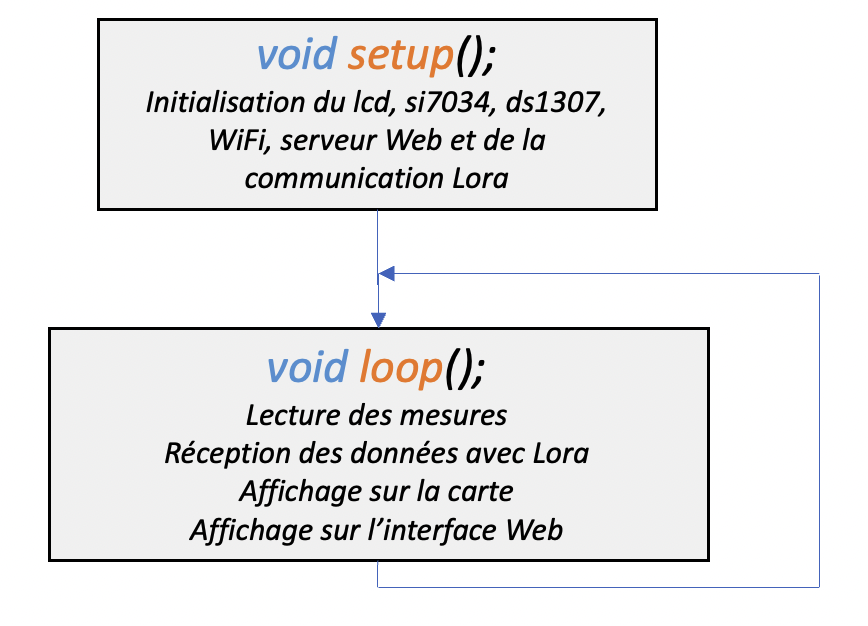
\includegraphics[width=.5\textwidth]{img/code/algo_main_server.png}
                    \caption{\label{fig:algo_main_server}Algorithme du main de la carte serveur}  
                \end{center}
            \end{figure}


\end{document}

